\chapter{Framework Architecture}
\label{chap:architecture}

This chapter presents the architecture of \emph{SysSimX}.
It begins with an overview of the layered structure and the design principles that guided its development.
The subsequent sections then describe the core abstractions that define the component interface, the system model, the execution algorithms, and the multi-model component concept.
Implementation details and verification of individual features are
deferred to Chapter~\ref{chap:implementation}.

\section{Architectural Overview}
\label{sec:architecture_overview}

Figure~\ref{fig:syssimx_architecture} shows the layered architecture of \syssimx{} and the delegation chain from user code through the framework to the external simulation backends.
The architecture is organized into four internal layers, adapter, core abstractions, system orchestration, and execution, each with a clearly defined responsibility.
Six design principles shaped this layering:
%
\begin{enumerate}[nosep]
  \item \textit{component-based decomposition,}
  \item \textit{tool-agnostic core with backend adapters,}
  \item \textit{separation of model and orchestration,}
  \item \textit{pluggable execution algorithms,}
  \item \textit{explicit and unit-aware interfaces, and}
  \item \textit{minimal required contract with optional capabilities.}
\end{enumerate}
%
Rather than discussing these principles in isolation, the following paragraphs introduce each layer of the architecture and explain the design decisions that motivated it.
The description proceeds from the bottom of Figure~\ref{fig:syssimx_architecture} upward, starting with the external tools and ending with the execution algorithms.

\begin{figure}[t]
  \centering
  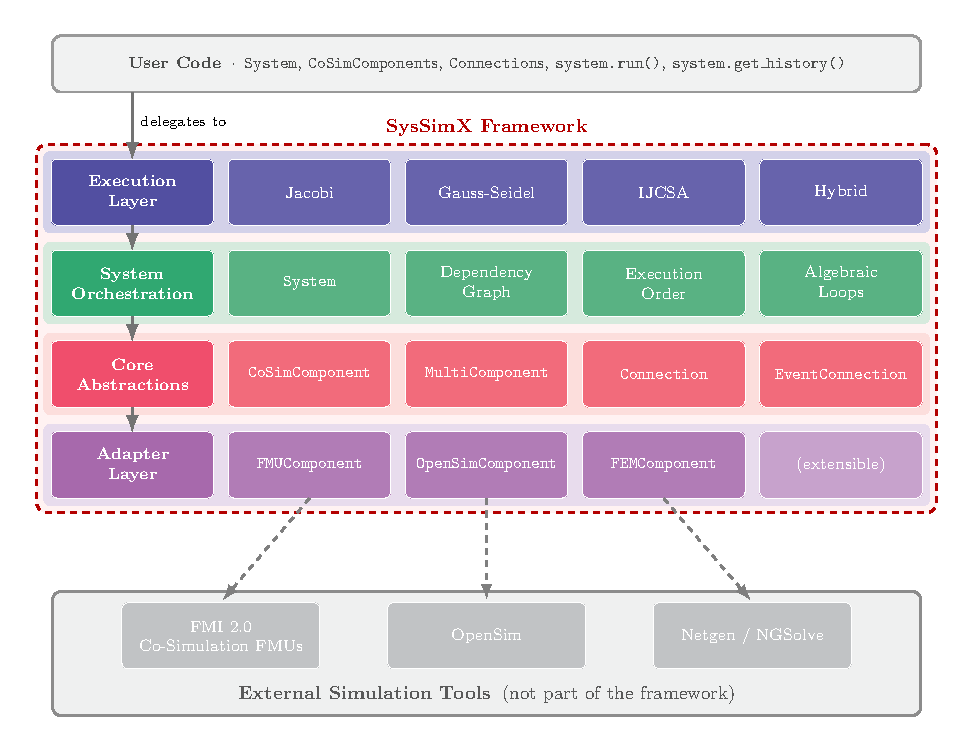
\includegraphics[width=\textwidth]{figures/4_architecture/syssimx_architecture.pdf}
  \caption{Layered architecture of the \syssimx{} framework.
  Solid arrows indicate the delegation direction between layers;
  dashed arrows indicate calls to external tool APIs across the
  framework boundary.}
  \label{fig:syssimx_architecture}
\end{figure}

\paragraph{External simulation tools.}
The simulation backends at the bottom of Figure~\ref{fig:syssimx_architecture} are not part of the framework.
They include FMI~2.0 Co-Simulation FMUs exported from equation-based modeling environments, OpenSim for musculoskeletal dynamics, and Netgen/NGSolve for finite element analysis.
Each tool provides its own solver, model representation, and programmatic Python interface.
The framework treats these tools as black-box backends and interacts with them exclusively through their respective APIs.

\paragraph{Adapter layer.}
The adapter layer wraps each tool-specific API in a class that implements the common  \texttt{CoSimComponent} interface.
\texttt{FMUComponent} maps FMI function calls to the component lifecycle.
\texttt{OpenSimComponent} wraps OpenSim in the same way.
For finite element models, \texttt{FEMComponent} marks the adapter slot but contributes minimal shared logic, since each FE model defines its own discretization, material law, and time integration scheme (Section~\ref{sec:impl_fem}).
As a result, every subsystem model, regardless of its origin, exposes the same interface for initialization, time stepping, input and output exchange, and state access.
This realizes the principle of a \emph{tool-agnostic core with backend adapters}.
All tool-specific code is confined to the adapter boundary, and the layers above can treat heterogeneous models uniformly.
The adapter layer is designed to be extensible. Additional backends can be integrated by providing a new adapter class without modifying the layers above.

\paragraph{Core abstractions.}
The core abstraction layer defines the modeling primitives of the framework.
The abstract base class \texttt{CoSimComponent} specifies the contract that every simulation component must satisfy. These are typed and unit-annotated input and output ports, a fixed lifecycle for initialization, stepping, and output evaluation, and optional hooks for direct-feedthrough declaration, event indicators, and state rollback.
This reflects two design principles.
First, \emph{component-based decomposition}, a system is represented as a set of interacting components that can be constructed, configured, and exchanged independently.
Second, \emph{minimal required contract with optional capabilities}, the component interface distinguishes between abstract methods that every component must implement and optional methods that enable participation in advanced framework features.
A simple component only needs to implement the core lifecycle methods.
Components that act as event sources must additionally implement state snapshot and rollback.
This keeps simple wrappers lightweight while allowing the framework to detect and exploit richer component capabilities where available.

Signal connections and event connections define the directed data flow and discrete event propagation between components.
\emph{Explicit and unit-aware interfaces} make coupling assumptions visible.
Each port carries a declared type and physical unit, and connections are validated for compatibility when they are added to the system.
The \texttt{MultiComponent} class extends this layer to the case where several interchangeable models represent the same physical subsystem, providing a single external interface while managing multiple internal realizations with consistent state synchronization.

\paragraph{System orchestration.}
The \texttt{System} class assembles components and connections into a complete co-simulation model.
It validates port compatibility, constructs the dependency graph, derives a topologically sorted execution order, identifies direct-feedthrough dependencies, and detects algebraic loops through strongly connected component analysis.
These structural properties are computed automatically during initialization and made available to the execution algorithms.
This layer embodies the \emph{separation of model and orchestration}.
Components are responsible for their own state integration and output evaluation, while the \texttt{System} class handles all system-level structural concerns.

\paragraph{Execution layer.}
The execution layer at the top of the framework contains the master algorithms that advance the coupled system in time.
An algorithm receives a \texttt{System} instance and steps all components from the current communication time~$t$ to~$t + \Delta t$, managing input propagation, output collection, and, where required, iterative resolution of algebraic loops or detection, localization, and handling of discrete events.
The same system model can be executed with different algorithms without modifying the component implementations or the system definition.
This realizes the principle of \emph{pluggable execution algorithms}.
The framework delegates all stepping logic to interchangeable algorithm objects, keeping numerical orchestration separate from model structure.

\paragraph{Supporting services.}
In addition to the main layers, the framework provides supporting services for unit handling, recording of port and component histories during simulation, and graph-based visualization of the system structure.

% The following sections describe each of the core abstractions in detail, beginning with the \texttt{CoSimComponent} interface.
\section{Core Abstractions}
\label{sec:architecture_core_abstractions}

This section describes the four core abstractions of \syssimx{}:
the component interface, the system model, the algorithm interface, and the multi-model component.
Together, they define the contracts on which the entire framework operates.
Their concrete realization and verification are discussed in
Chapter~\ref{chap:implementation}.

\subsection{CoSimComponent Interface}
\label{sec:architecture_cosimcomponent}

The \texttt{CoSimComponent} interface defines the architectural contract for simulation components in \syssimx{}.
It separates backend-specific model behavior from framework-level orchestration.
All components expose the same interface for initialization, stepping, data exchange, and result collection.
This uniform contract follows from the co-simulation formulation in Section~\ref{sec:232_cosim_formulation}.

The master algorithms require a component interface with four properties.
Components must expose typed and unit-aware ports.
They must support a common lifecycle for initialization and stepping.
They must declare the input-output dependencies needed for structural analysis.
Components that participate in hybrid scenarios must also provide the state handling needed for rollback.
Figure~\ref{fig:cosimcomponent_architecture} summarizes this interface.

\begin{figure}[t]
  \centering
  \vspace{-1em}
  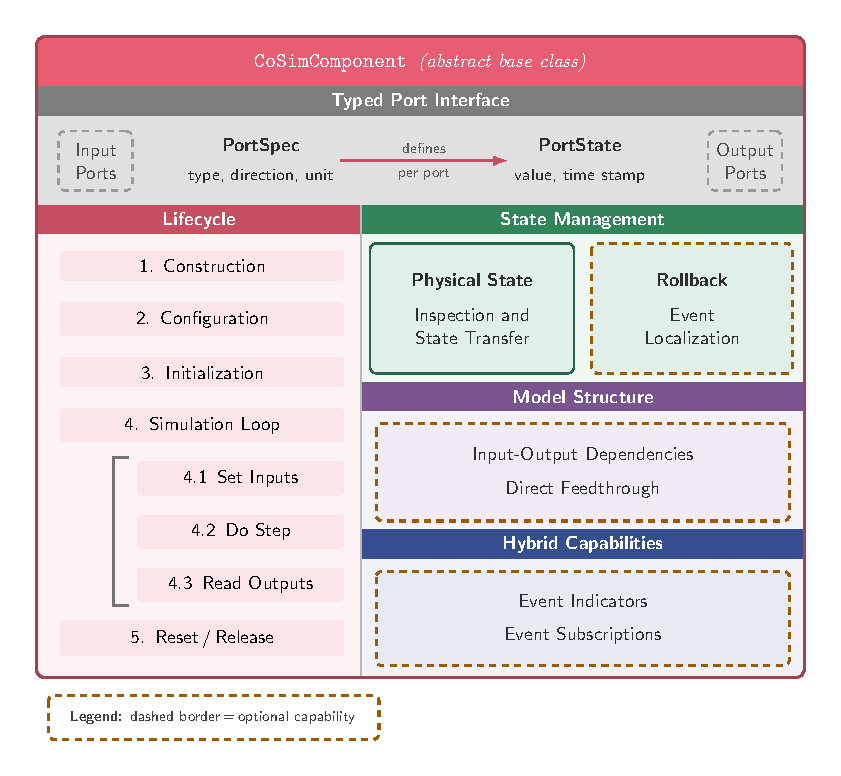
\includegraphics[width=0.95\textwidth]{figures/4_architecture/cosimcomponent.pdf}
  \vspace{-1em}
  \caption{Architectural overview of the \texttt{CoSimComponent} interface.
  The interface combines typed ports, a common lifecycle, state handling, and optional capabilities for structural analysis and hybrid co-simulation.}
  \vspace{-0.5em}
  \label{fig:cosimcomponent_architecture}
\end{figure}

\paragraph{Typed Port Interface.}
A component exposes its system interface through typed input and output ports.
Each port carries a declared data type and an optional physical unit.
These declarations make coupling assumptions explicit at the interface level.
They also allow the framework to validate type compatibility and unit consistency when connections are established, as described in Section~\ref{sec:architecture_system_connections}.

\paragraph{Lifecycle and Inversion of Control.}
The interface prescribes a common lifecycle for all components.
A component is constructed, configured, initialized at the simulation start time, stepped during the simulation loop, and reset or finalized after use.
The framework owns this lifecycle order.
Backend-specific subclasses provide the model operations that are called inside this order.

This inversion of control keeps framework concerns in one place.
Port-state management, time bookkeeping, history recording, and capability checks are handled uniformly.
Backend wrappers can focus on model-specific initialization, stepping, and output evaluation.

\paragraph{Declared Structural and Hybrid Metadata.}
The component interface also exposes metadata needed by the system-level orchestration.
The direct-feedthrough declaration states which outputs can depend on which inputs within the same communication step.
The \texttt{System} abstraction uses this information together with the connection structure to derive the execution constraints described in Section~\ref{sec:233_cosim_structural_analysis}.

Hybrid components can additionally expose event indicators and event subscriptions.
Event indicators allow an algorithm to detect and localize discrete events.
Event subscriptions define which components must receive an event after it has been detected.

\paragraph{State Handling.}
The interface separates physical state transfer from rollback state transfer.
Physical state transfer exports semantically meaningful quantities such as positions, velocities, or mode indicators.
It is used for inspection and for synchronization between alternative models of the same subsystem.

Rollback state transfer captures and restores the internal solver state of a component.
It is used during hybrid event handling, where the simulation may have to return to an earlier time and re-advance.
The two mechanisms are separated because rollback state is tool-specific, while physical state must remain meaningful across model representations.

\paragraph{Opt-in Capabilities.}
Components do not have to support every advanced capability.
The lifecycle operations are mandatory.
Physical state transfer, rollback, zero-step output evaluation, event indicators, and event handling are optional.
This keeps simple components lightweight and limits additional complexity to components that participate in strongly coupled or hybrid scenarios.
\subsection{System and Connections}
\label{sec:system_connections}

The \texttt{System} class represents a complete co-simulation model.
It collects the participating components, stores the connections between them, and provides the structural context required for orchestration.
In this way, the definition of individual subsystem models is kept separate from the definition of the coupled system.
Figure~\ref{fig:system_architecture} illustrates this separation: the left panel shows a system as defined by the user, while the right panel shows the structural information the framework derives during initialization.

\begin{figure}[htbp]
  \centering
  \vspace{-1em}
  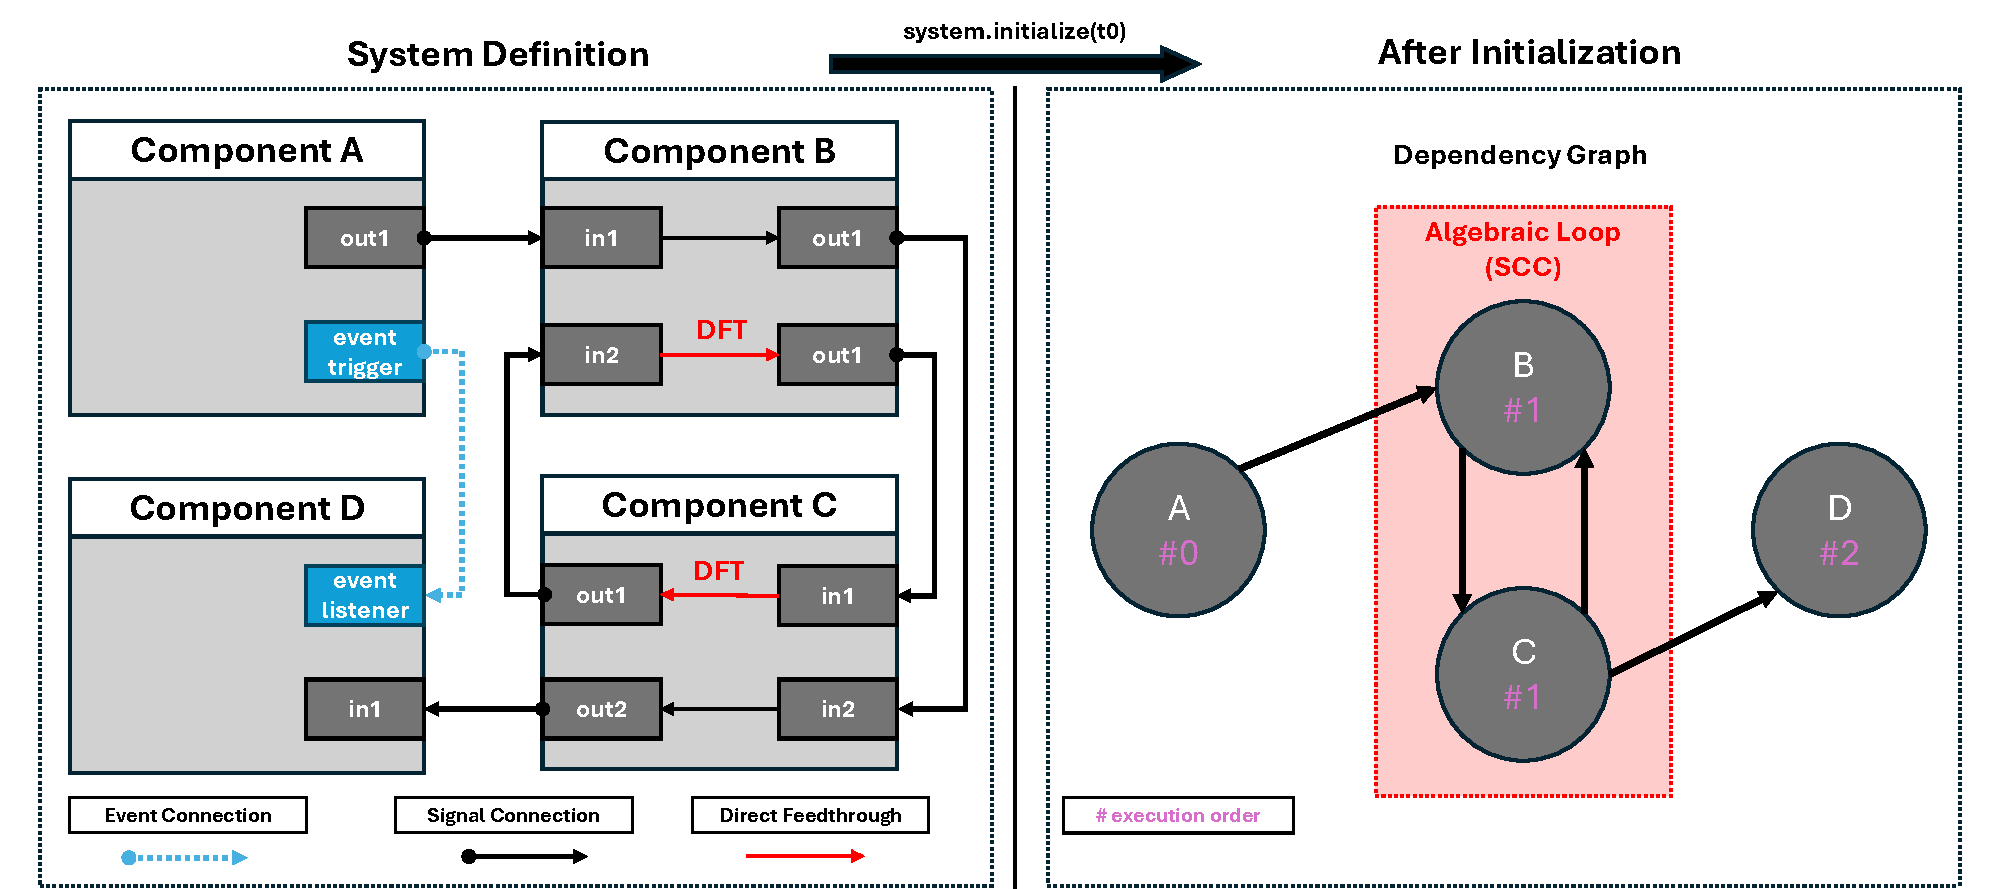
\includegraphics[width=\textwidth]{figures/4_architecture/system_architecture.pdf}
  \vspace{-1em}
  \caption{System definition and initialization. The left panel shows the user-defined system model with four components, their typed ports, signal connections (solid arrows), an event connection (dashed blue), and direct-feedthrough paths (solid red). The right panel shows the result of \texttt{system.initialize(t0)}: the framework derives a dependency graph, computes a topologically sorted execution order (\#), and identifies algebraic loops as strongly connected components (shaded region).}
  \vspace{-0.5em}    
  \label{fig:system_architecture}
\end{figure}

Two types of connections are supported.
A signal connection defines a directed data flow from an output port of a source component to an input port of a destination component.
An event connection routes a named event from a source component to a handler method in a destination component, enabling cross-component discrete interactions such as mode changes or contact triggers.
Both connection types are visible in Figure~\ref{fig:system_architecture} (left): solid arrows denote signal connections, while the dashed arrow represents an event connection.
When a connection is added, the \texttt{System} validates that the referenced ports exist and that the connected ports are type- and unit-compatible.

From the registered components and connections, the \texttt{System} builds a dependency graph in which components form the nodes and directed connections form the edges.
This graph is the basis for the structural analysis performed during initialization: the framework derives a topologically sorted execution order, identifies direct-feedthrough dependencies, and detects algebraic loops.
As shown in Figure~\ref{fig:system_architecture} (right), components~B and~C form a strongly connected component due to their mutual direct-feedthrough dependencies, which the framework flags as an algebraic loop.
The details of these analyses are discussed in Chapter~\ref{chap:implementation}; at the architectural level, it is sufficient to note that they are computed automatically and made available to the execution algorithms.

The \texttt{System} class does not implement a stepping scheme itself.
Instead, it holds a reference to an \texttt{Algorithm} object and delegates the simulation loop to it.

\subsection{Algorithm Interface}
\label{sec:arch_algorithm}

The algorithm interface separates the assembled system structure from the execution strategy.
The \texttt{System} owns the components, connections, and structural context.
An algorithm owns the procedure that advances this system in time.
This separation allows the same system definition to be executed with different coordination schemes.

Each algorithm advances the coupled system in macro steps of size~$\Delta t$.
During a macro step, it coordinates input propagation, component stepping, output collection, and any additional treatment required by the system structure.
Explicit algorithms evaluate components according to the available execution order.
Algebraic-loop algorithms add coupled treatment for instantaneous dependencies.
Hybrid algorithms add event detection, event localization, and event dispatch.

All algorithms use the same component and system interfaces.
The user can therefore change the execution strategy without changing the component implementations or the system definition.
The concrete algorithms and their numerical procedures are described in Sections~\ref{sec:impl_algorithms} through~\ref{sec:impl_hybrid}.
\subsection{Multi-Model Component}
\label{sec:architecture_multicomponent}

The \texttt{MultiComponent} abstraction extends the component interface to several interchangeable model realizations of one physical subsystem.
It exposes one public component interface to the surrounding \texttt{System} and delegates execution to one active internal model.
This supports runtime switching between models with different fidelity levels or modeling approaches.

Figure~\ref{fig:multi_component} shows the public interface, the internal model registry, and the switching-support responsibilities.

\begin{figure}[t]
  \centering
  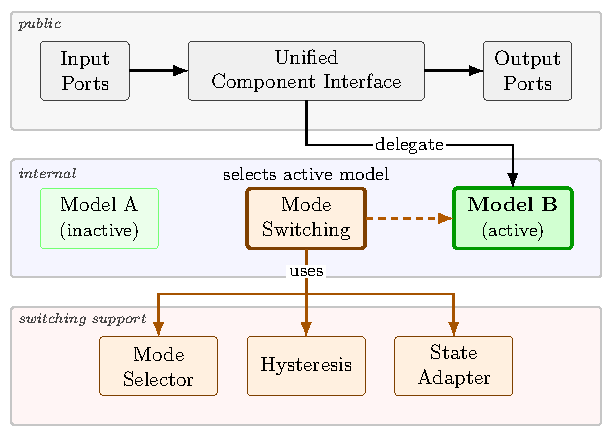
\includegraphics[width=0.7\textwidth]{figures/4_architecture/multi_model.pdf}
  \caption[Architectural view of the \texttt{MultiComponent} abstraction]{Architectural view of the \texttt{MultiComponent} abstraction.
  The wrapper exposes one unified component interface and delegates execution to one active model from a registered set.
  A mode selector, hysteresis, and state adapter together change the active model when the switching criteria require it.}
  \label{fig:multi_component}
\end{figure}

At any point in time, exactly one internal model is active.
The active model provides the outputs exposed by the wrapper and receives the delegated lifecycle and stepping calls.
Inactive models remain registered inside the wrapper so that they can become active later without changing the surrounding system structure.

A switch changes the active model.
The mode selector determines the requested model from the switching criteria defined by the concrete component.
Hysteresis enforces a minimum dwell time between consecutive switches and suppresses rapid changes near switching boundaries.
The state adapter maps the physical state exported by the outgoing model to a representation accepted by the incoming model.

The abstraction separates model choice from system assembly.
The surrounding \texttt{System} connects only to the public interface of the \texttt{MultiComponent}.
The implementation details of port unification, state transfer, and switching are described in Section~\ref{sec:impl_multi_model}.